\documentclass[12pt]{Qual}
\usepackage{preamble}

\name{Kayla Orlinsky}
\course{Complex Analysis Exam}
\term{Spring 2011}
\hwnum{Spring 2011}

\begin{document}

\begin{problem} $\,$
Evaluate $$\int_0^\infty\frac{\log x}{(x^2+1)^2}dx$$
\end{problem}


\begin{solution}$\,$
We will use ``Ol' Faithful'' the contour around the upper half plane avoiding the origin since every branch cut of $\log x$ intersects $0$.

Then we take any branch which does not intersect the upper half plane (including the real line).
\begin{center}
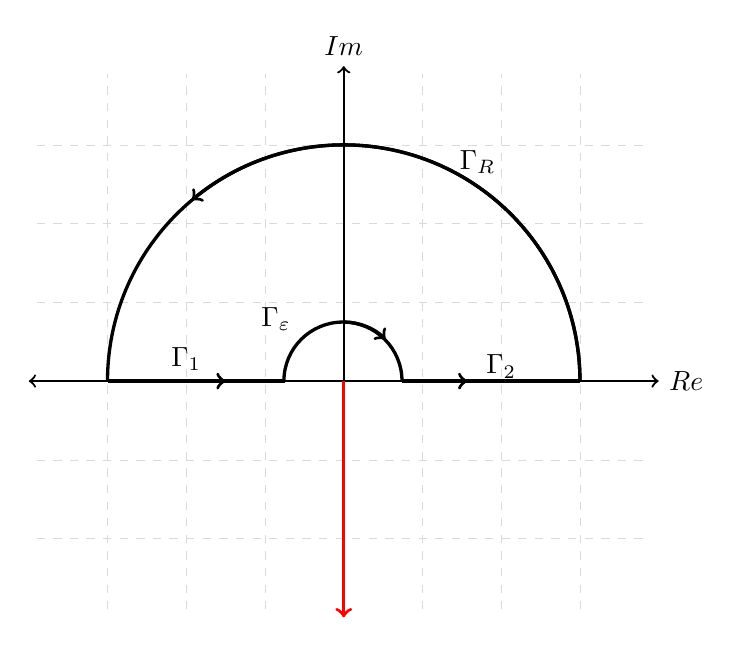
\begin{tikzpicture}
\draw[help lines, color=gray!30, dashed] (-3.9,-2.9) grid (3.9,3.9);
\draw[->,very thick] (3,0) arc (0:130:3cm);
\draw[very thick] (3,0) arc (0:180:3cm) node[above,yshift=2.5cm,xshift=4.7cm]{$\Gamma_R$};
\draw[->,very thick] (0,0.75) arc (90:45:0.75cm);
\draw[very thick] (0.74,0) arc (0:180:0.75cm) node[above,yshift=0.5cm,xshift=-0.1cm]{$\Gamma_\varepsilon$};
\draw[->,very thick] (0.74,0) -- (1.57,0);
\draw[very thick] (0.75,0) -- (3,0) node[above,yshift=-0.1cm,xshift=-1cm]{$\Gamma_2$};
\draw[->,very thick] (-3,0) -- (-1.5,0);
\draw[very thick] (-0.74,0) -- (-3,0) node[above,yshift=0cm,xshift=1cm]{$\Gamma_1$};
\draw[<->, thick] (-4,0)--(4,0) node[right]{$Re$};
\draw[->, thick] (0,0)--(0,4) node[above]{$Im$};
\draw[->,very thick,red] (0,0) -- (0,-3);
\end{tikzpicture}
\end{center}

Let \begin{align*}
    I_1&=\int_{\Gamma_1}\frac{\log z}{(z^2+1)^2}dz\\
    I_2&=\int_{\Gamma_2}\frac{\log z}{(z^2+1)^2}dz\\
    I_\varepsilon&=\int_{\Gamma_\varepsilon}\frac{\log z}{(z^2+1)^2}dz\\
    I_R&=\int_{\Gamma_R}\frac{\log z}{(z^2+1)^2}dz
\end{align*}

For the next computation we refer to the following triangle:
\begin{center}
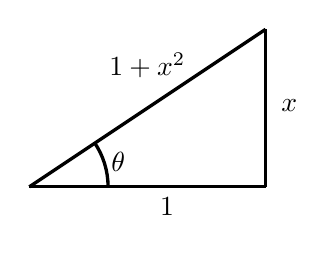
\begin{tikzpicture}
\draw[very thick] (1,0) arc (0:34:1cm) node[above,xshift=0.3cm, yshift=-0.5cm]{$\theta$};
\draw[very thick] (0,0) -- (3,0) node[below,xshift=-1.25cm]{$1$};
\draw[very thick] (3,0) -- (3,2) node[below,xshift=0.3cm,yshift=-0.75cm]{$x$};
\draw[very thick] (0,0) -- (3,2) node[above,xshift=-1.5cm,yshift=-0.75cm]{$1+x^2$};
\end{tikzpicture}
\end{center}

\begin{align*}
    I_1&=\int_{\Gamma_1}\frac{\log z}{(z^2+1)^2}dz\\
    &=\int_{-R}^{-\varepsilon}\frac{\log x}{(x^2+1)^2}dx\\
    &=\int_R^\varepsilon\frac{-\log(-x)}{(x^2+1)^2}dx\\
    &=\int_\varepsilon^R\frac{\log x+i\pi}{(x^2+1)^2}dx\qquad \log(-x)=\log x+i\pi\\
    &=I_2+\int_\varepsilon^R\frac{i\pi}{(x^2+1)^2}dx\\
    &=I_2+i\pi\int_\varepsilon^R\frac{\sec^2\theta}{(\tan^2\theta+1)^2}d\theta\qquad x=\tan\theta\\
    &=I_2+i\pi\int_\varepsilon^R\frac{\sec^2\theta}{\sec^4\theta}d\theta\\
    &=I_2+i\pi\int_\varepsilon^R\frac{1}{\sec^2\theta}d\theta\\
    &=I_2+i\pi\int_\varepsilon^R\cos^2\theta d\theta\\
    &=I_2+i\pi\frac{1}{2}\int_\varepsilon^R1+\cos(2\theta) d\theta\\
    &=I_2+\frac{i\pi}{2}\left[\theta+\frac{1}{2}\sin(2\theta)\right]\Big|_{x=\varepsilon}^R\\
    &=I_2+\frac{i\pi}{2}\left[\tan^{-1}(x)+\sin(\theta)\cos(\theta)\right]\Big|_{x=\varepsilon}^R\\
    &=I_2+\frac{i\pi}{2}\left[\tan^{-1}(x)+\frac{x}{(x^2+1)^2}\right]\Big|_{x=\varepsilon}^R\\
    &\to I_2+\frac{i\pi}{2}\left[\frac{\pi}{2}\right]\qquad\text{as }\varepsilon\to0,R\to\infty\\
    &=I_2+i\frac{\pi^2}{4}
\end{align*}



Now, \begin{align*}
    |I_R|&=\left|\int_{\Gamma_R}\frac{\log z}{(z^2+1)^2}dz\right|\\
    &\le \int_{\Gamma_R}\frac{|\log z|}{|z^2+1|^2}|dz|\\
    &\le\int_{\Gamma_R}\frac{|z|+C}{|z^2+1|^2}dz\tag{1}\\
    &\le\int_{\Gamma_R}\frac{R+C}{|z|^2}dz\tag{2}\\
    &=\int_{\Gamma_R}\frac{R+C}{R^2}dz\to0\qquad\text{as }R\to\infty
\end{align*}

Note that (1) comes from $$|\log z|=\sqrt{(\log |z|)^2+(\arg(z))^2}\le \sqrt{(\log|z|)^2}+C=\log|z|+C\le |z|+C$$ for $C$ sufficiently large with respect to the maximal possible argument of $z$, which is $\frac{3\pi}{2}.$

And (2) comes from $|z^2+1|^2\ge |z^2+1|\ge |z^2|$ for $|z|$ sufficiently large.

Finally, \begin{align*}
    |I_\varepsilon|&=\left|\int_{\Gamma_\varepsilon}\frac{\log z}{(z^2+1)^2}dz\right|\\
    &\le\int_\pi^0\frac{|\log(\varepsilon e^{i\theta})||i\varepsilon e^{i\theta}|}{|\varepsilon^2e^{2i\theta}+1|^2}d\theta\\
    &\le\int_\pi^0\frac{\varepsilon(|\log \varepsilon|+|\theta|)}{|\varepsilon^2e^{2i\theta}+1|^2}d\theta\to0\qquad\varepsilon\to0
\end{align*}

Note that \begin{align*}
    \lim_{\varepsilon\to0}\frac{\varepsilon(|\log \varepsilon|+|\theta|)}{|\varepsilon^2e^{2i\theta}+1|}&=\left(\lim_{\varepsilon\to0}\frac{|\log \varepsilon|}{\frac{1}{\varepsilon}}\right)\left(\lim_{\varepsilon\to0}\frac{1}{|\varepsilon^2e^{2i\theta}+1|^2}\right)+\lim_{\varepsilon\to0}\frac{\varepsilon|\theta|}{|\varepsilon^2e^{2i\theta}+1|^2}\\
    &=\lim_{\varepsilon\to0}\frac{\frac{1}{\varepsilon}}{\frac{-1}{\varepsilon^2}}\cdot1+0\\
    &=\lim_{\varepsilon\to0}-\varepsilon=0
\end{align*} by L'Hopital's rule.

Therefore, by the residue theorem, \begin{align*}
    \lim_{\varepsilon\to0}\lim_{R\to\infty}I_1+I_2+I_\varepsilon+I_R&=2\pi i\res_{z=i}\frac{\log z}{(z^2+1)^2}\\
    &=2\pi i\frac{d}{dz}\frac{\log z}{(z+i)^2}\Big|_{z=i}\\
    &=2\pi i\frac{\frac{(z+i)^2}{z}-2(z+i)\log z}{(z+i)^4}\Big|_{z=i}\\
    &=2\pi i\frac{\frac{(2i)^2}{i}-2(2i)\log i}{(2i)^4}\\
    &=2\pi i\frac{4i-4i\frac{\pi}{2}i}{16}\\
    &=-\frac{\pi}{2}\left(1-\frac{\pi}{2}i\right)\\
    &=\frac{\pi^2}{4}i-\frac{\pi}{2}\\
    \lim_{\varepsilon\to0}\lim_{R\to\infty}I_1+I_2+I_\varepsilon+I_R&=2I_1+\frac{\pi^2}{4}i\\
    \implies I_1&=\frac{1}{2}\left(\frac{\pi^2}{4}i-\frac{\pi}{2}-\frac{\pi^2}{4}i\right)\\
    &=-\frac{\pi}{4}
\end{align*}
\end{solution}
\newpage

\begin{problem} $\,$
\begin{enumerate}[label=(\alph*)]
    \item Suppose that $u_1,u_2,...,u_n$ and $u_1^2+\cdots+u_n^2$ are harmonic functions on a connected open set $D$. Show that each function $u_r$ ($1\le r\le n$) is constant.
    \item A function $f:D\to\mathbb{C}$ with $f(x+iy)=u(x,y)+iv(x,y)$ is said to be complex harmonic if the real valued functions $u$ and $v$ are harmonic. Show that if $f(x+iy)$ and $(x+y)f(x+iy)$ are both complex harmonic then $f$ is analytic.

    \boxed{\textbf{TYPO}:}\textit{ This question does not make sense unless we assume that $(x+iy)f(x+iy)$ is complex harmonic.}
\end{enumerate}
\end{problem}


\begin{solution}$\,$
\begin{enumerate}[label=(\alph*)]
    \item Note that \begin{align*}
        \frac{\partial}{\partial x}u^2&=2u\frac{\partial u}{\partial x}\\
        \frac{\partial^2}{\partial x^2}u^2&=\frac{\partial}{\partial x}\left(2u\frac{\partial u}{\partial x}\right)\\
        &=2\left(\frac{\partial u}{\partial x}\right)^2+2u\frac{\partial^2 u}{\partial x^2}\\
         \frac{\partial^2}{\partial x^2}u^2+ \frac{\partial^2}{\partial y^2}u^2&=2\left(\frac{\partial u}{\partial x}\right)^2+2u\frac{\partial^2 u}{\partial x^2}+2\left(\frac{\partial u}{\partial y}\right)^2+2u\frac{\partial^2 u}{\partial y^2}\\
         &=2\left[2\left(\frac{\partial u}{\partial x}\right)^2+2\left(\frac{\partial u}{\partial y}\right)^2\right]
    \end{align*} which is $0$ if and only if $\frac{\partial u}{\partial x}=\frac{\partial u}{\partial y}=0$.

    Therefore, since differentiation is a linear operation, $u_1^2+\cdots+u_n^2$ is harmonic if and only if $$\frac{\partial u_k}{\partial x}=\frac{\partial u_k}{\partial y}\qquad\text{ for all }k.$$ Namely, $u_k=c_k$ for some $c_k$ constant for all $k.$

    \item We will write $u_x=\frac{\partial}{\partial x}u.$

    \boxed{\text{Original Hypothesis}} Now, because $(x+y)f(x+iy)$ is complex harmonic, \begin{align*}
        0&=\frac{\partial^2}{\partial x^2}(x+y)u+\frac{\partial^2}{\partial y^2}(x+y)u\\
        &=\frac{\partial}{\partial x}\left[u+(x+y)u_x\right]+\frac{\partial}{\partial y}\left[u+(x+y)u_y\right]\\
        &=u_x+u_x+(x+y)u_{xx}+u_y+u_y+(x+y)u_{yy}\\
        &=2u_x+2u_y
    \end{align*} since $f(x+iy)$ is complex harmonic so $u_{xx}=-u_{yy}.$

    Therefore, $u_x=-u_y$ and similarly, $v_x=-v_y$.

    However, to obtain the final solution, it is necessary to assume that $(x+iy)f(x+iy)$ is complex harmonic, instead of $(x+y)f(x+iy)$.

    \boxed{\text{Assuming }(x+iy)f(x+iy)\text{ is complex harmonic}} Now, $$(x+iy)f(x+iy)=(x+iy)(u+iv)=xu-yv+i(yu+xv)$$ and so the real part being harmonic now implies that \begin{align*}
        0&=\frac{\partial^2}{\partial x^2}(xu-yv)+\frac{\partial^2}{\partial y^2}(xu-yv)\\
        &=\frac{\partial}{\partial x}\left[u+xu_x-yv_x\right]+\frac{\partial}{\partial y}\left[xu_y-v-yv_y\right]\\
        &=u_x+u_x+xu_{xx}-yv_{xx}+xu_{yy}-v_y-v_y-yv_{yy}\\
        &=2u_x-2v_y
    \end{align*}

    since $f(x+iy)$ is complex harmonic so $xu_{xx}+xu_{yy}=0$ and similarly, $-yv_{xx}-yv_{yy}=0.$

    Now finally, the complex part of $f(x+iy)$ is harmonic and so \begin{align*}
        0&=\frac{\partial^2}{\partial x^2}(yu+xv)+\frac{\partial^2}{\partial y^2}(yu+xv)\\
        &=\frac{\partial}{\partial x}\left[yu_x+v+xv_x\right]+\frac{\partial}{\partial y}\left[u+yu_y+xv_y\right]\\
        &=yu_{xx}+v_x+v_x+xv_{xx}+u_y+u_y+yu_{yy}+xv_{yy}\\
        &=2v_x+2u_y
    \end{align*}

    and so $u_x=v_y$ and $u_y=-v_x$. Therefore, by Cauchy-Riemann, $f(x+iy)$ is analytic.
\end{enumerate}
\end{solution}
\newpage

\begin{problem} $\,$
Let $f:D\to D$ be an analytic function on a bounded domain $D$ with $0\in D$. Assume $f(0)=0$ and $|f'(0)|<1$. Let $F_n(z)=f\circ \cdots\circ f(z)$ ($n$-times). Show that $F_n(z)\to0$ as $n\to\infty$ uniformly on compact subsets of $D$. Hint: consider first the behavior of $F_n$ on a small neighborhood of $0.$
\end{problem}


\begin{solution}$\,$
Since $$\left|\lim_{z\to0}\frac{f(z)-f(0)}{z-0}\right|=\lim_{z\to0}\frac{|f(z)|}{|z|}=|f'(0)|,$$ we have that for all $\varepsilon>0$, there exists $\delta>0$ such that $$\varepsilon>\left|\frac{f(z)}{z}-f'(0)\right|\ge\frac{|f(z)}{|z|}-|f'(0)|\qquad |z|<\delta.$$

Therefore, $$\frac{|f(z)|}{|z|}<\varepsilon+|f'(0)|.$$ Since $\varepsilon>0$ was arbitrary and $|f'(0)|<1$, there exists $0<\rho<1$ such that $$\frac{|f(z)|}{|z|}\le\rho<1$$ for all $|z|<\delta.$

Note, that since $D$ is the domain of an analytic function we may take it to be connected and open, so we can take $\delta$ such that $B_\delta(0)\subset D$. Namely, we have that $|f(z)|\le \rho|z|$ for all $z\in B_\delta(0)\subset D.$

Finally, since $\rho<1$, $\rho z\in B_\delta(0)$ for all $z\in B_\delta(0).$

Thus, $$|f\circ\cdots\circ f(z)|\text{ (}n\text{-times) }\le |f\circ\cdots\circ f(\rho z)|\text{ (}n-1\text{-times) }=|f\circ\cdots\circ f(\rho^2 z)\text{ (}n-2\text{-times) }\le\cdots\le \rho^n|z|.$$

Therefore, $$\lim_{n\to\infty}|f\circ\cdots\circ f(z)|\text{ (}n\text{-times) }\le \lim_{n\to\infty}\rho^n|z|=0$$ for all $z\in B_\delta(0)$ since $\rho<1.$

Next, assume that $K\subset D$ is compact. By Cauchy, because $D$ is bounded, and $f:D\to D$, there exists $M$ such that $|f(z)|\le M$ for all $z\in D.$

Namely, $|F_n(z)|\le M$ for all $z\in D.$ Therefore, by Montel's Theorem, $\{F_n\}$ define a normal family on $D.$

Therefore, for every $z\in D$, there exists a subsequence $\{F_{n_k}\}$ of $\{F_n\}$ such that $F_{n_k}\to F$ uniformly on compact subsets $K\subset D$, for some analytic function $F:D\to D.$

However, $F_{n_k}|_{B_\delta(0)}\to0$ uniformly, which implies that $F|_{B_\delta(0)}=0$. Since $F$ is analytic, its zeros must be isolated, so $F=0$ for every $z$ in a ball implies that $F\equiv0$ is identically $0$ on $D.$

Namely, for each $K\subset D$ compact, there exists a subsequence $\{F_{n_k}\}$ which converges uniformly to $0$ on $K.$

Finally, to show that the whole sequence converges to $0$ on $K,$ we note that for all $\varepsilon>0$, there exists $N$ such that $$|F_{n_k}|<\varepsilon\qquad\text{ for all }n_k\ge N\text{ in the subsequence}.$$

However, from the above, if $|F_{n_k}(z)|<\varepsilon,$ then $$|f(F_{n_k}(z))|\le \rho|F_{n_k}(z)|<\rho\varepsilon<\varepsilon\qquad \rho<1$$ and so, since $f\circ F_{n_k}(z)=F_{n_k+1}(z)$, we have that $|F_n(z)|<\varepsilon$ for all $n\ge N$.

Namely, $F_n\to0$ uniformly on $K$
\end{solution}
\newpage





\begin{problem} $\,$
Starting with the definition

``$f$ is analytic on a set $G$ if $\lim_{z\to z_0}\frac{f(z)-f(z_0)}{z-z_0}$ exists for all $z_0\in G.$''

describe the sequence of intermediate results required to obtain the following theorem:

``Suppose $f$ and $g$ are both analytic on a connected open set $G$ and there is a convergent sequence $z_n$ with limit $z_\infty\in G$ such that $f(z_n)=g(z_n)$ for all $n.$ Then $f=g$ on $G.$''

You do not need to prove any of the intermediate results, but you should give a brief indication of how each result is used to obtain the next one.
\end{problem}


\begin{solution}$\,$
\begin{center}
    \boxed{\textbf{THIS QUESTION IS TERRIBLE. Proofs will be provided for the sake of learning...}}
\end{center}
\begin{enumerate}
    \item Since $f$ and $g$ are analytic, $f-g$ is analytic by Cauchy-Riemann.
    \item The zeros of analytic functions are isolated. Although we used this freely in \textbf{Problem 3}, for the sake of understanding we prove this as a claim.
    \begin{claim} The zeros of an analytic function are isolated.
    \begin{proof} Let $h$ be an analytic function and let $z_0$ be a zero of $h.$ Then, because $h$ is analytic, we can develop its Taylor series about $z_0$ in $B_R(z_0)$ for some $R>0$. Namely, $$h(z)=\sum_{n=0}^\infty a_n(z-z_0)^n.$$

    Now, since $z_0$ is a zero of $h$, $a_0=0$, and so WLOG, we can take $N$ to be the largest integer such that $a_n=0$ for all $0\le n<N$ and $a_N\not=0$. Then, $$h(z)=\sum_{n=N}^\infty a_n(z-z_0)^n=\sum_{n=0}^\infty a_{n+N}(z-z_0)^{n+N}=(z-z_0)^N\sum_{n=0}^\infty a_{n+N}(z-z_0)^n$$

    Therefore, $h(z)=(z-z_0)^Nk(z)$ with $k(z)=\sum_{n=0}^\infty a_{n+N}(z-z_0)^n$ also an analytic function on $B_R(z_0)$. Furthermore, $k(z_0)=a_N\not=0$ by assumption.

    Thus, because $k$ is analytic, it is continuous, and because $k(z_0)$ non-zero, there exists a $\delta>0$ such that $$|k(z)-a_N|<\frac{|a_N|}{2}\qquad |z-z_0|<\delta$$ and so $k(z)\not0$ on $B_\delta(z_0)$.

    Namely, $z_0$ must be an isolated singularity of $h$.
    \end{proof}
    \end{claim}
    \item Because $f-g$ is analytic (by 1.) and $f-g=0$ on a sequence in $G$, the zeros of $f-g$ cannot be isolated. This is because limit points are not isolated by definition.

    Therefore, assuming that $f-g$ is not identically $0$ contradicts 2. and so $f-g\equiv 0$ on $G$. Thus, $f=g$ on $G.$
\end{enumerate}
\end{solution}


\end{document}
